\documentclass[11pt,a4paper]{amsart}
\usepackage[utf8]{inputenc}
\usepackage[T1]{fontenc}
\usepackage{lmodern}
\usepackage{amsmath,amssymb,amsthm}
\usepackage{booktabs}
\usepackage{array}
\usepackage{placeins}
\usepackage{graphicx}
\usepackage[margin=2.5cm]{geometry}
\usepackage{xcolor}
\usepackage[colorlinks=true,linkcolor=blue!50!black,citecolor=blue!50!black,urlcolor=blue!50!black]{hyperref}

\newtheorem{theorem}{Theorem}
\newtheorem{lemma}[theorem]{Lemma}
\newtheorem{proposition}[theorem]{Proposition}
\newtheorem{corollary}[theorem]{Corollary}
\theoremstyle{remark}
\newtheorem*{remark}{Remark}

\newcommand{\cP}{\mathcal P}
\newcommand{\cE}{\mathcal E}

\title[Exponents and windows in \lq\lq When the sieve works\rq\rq]{A note on the smooth-number exponents and
the additive windows in \texorpdfstring{\lq\lq When the sieve works\rq\rq}{"When the sieve works"}}
\thanks{Code and data are archived at Zenodo, \href{https://doi.org/10.5281/zenodo.24297466}{doi:10.5281/zenodo.24297466};\\ repository: \href{https://github.com/Ruqing1963/gkm-2015-when-sieve-works-audit}{github.com/Ruqing1963/gkm-2015-when-sieve-works-audit}.}
\author{Ruqing Chen}
\address{GUT Geoservice Inc., Montreal, Canada}
\email{ruqing@hotmail.com}
\date{November 16, 2026}
\subjclass[2020]{11N25, 11N35, 11B13}
\keywords{smooth numbers, sieve, Rankin's method, sumsets, additive combinatorics}

\begin{document}
\begin{abstract}
We check four technical points in \emph{When the sieve works} by A.~Granville, D.~Koukoulopoulos and
K.~Matom\"aki (Duke Math.\ J.\ \textbf{164} (2015), 1935--1969). (i) The proof of Proposition~2.6 bounds a sum over
$a\in(\sqrt x,x]$ by $e^{O(v)}(v\log v)^{-v/2}$ where $v=\log x/(2.5\log\log x)$. This is
$x^{-1/5+o(1)}$, not $\ll x^{-1/3}$ as in (2.7). The rescaling in (2.8) then gives $x^{-1/10+o(1)}$, not
$x^{-1/6}$. The method yields Proposition~2.6 with $x^{-1/6}$ replaced by $x^{-1/8+\epsilon}$, and its
qualitative conclusion is unchanged. (ii) Lemma~8.5, stated without proof, is false as printed: for $u=1$, $v=4$,
$w=1$ and $T=(0.6,0.7)$ its left-hand side vanishes for every $\ell$. The window must have width $1/u$, or
$T\subset(\frac1{ev},\frac1v]$. We prove both versions; the second is the one needed for
Proposition~8.4. (iii) The proof of Hypothesis P $\Rightarrow$ Hypothesis A can produce primes outside
$(x^{1/ev},x^{1/u}]$; removing at most two elements of $A$ repairs it. (iv) An inequality in the proof of
Proposition~8.1 fails as $\sigma\to1$, but the conclusion holds as stated. No main result is affected.
\end{abstract}
\maketitle

\section{Introduction}

The paper \cite{GKMat} of Granville, Koukoulopoulos and Matom\"aki determines when the sieve upper bound
$\Psi(x;\cP)\ll x\prod_{p\in\cE,\,p\le x}(1-1/p)$ is attained, where $\cP$ is a set of primes, $\cE$ its
complement, and $\Psi(x;\cP)$ counts the integers $\le x$ all of whose prime factors lie in $\cP$. The
proof passes through Hypotheses P, A and T (Sections~3--4) and additive combinatorics (Sections~5--7).
Section~2 contains a converse result (Proposition~2.6), and Section~8 further consequences. We check the
explicit exponents and windows in these parts. Page numbers refer to the arXiv version
(arXiv:1205.0413v2, 26 pages). All numbers below were recomputed by a program provided as supplementary
material. Each repair is local. Proposition~2.6 keeps a power saving, Proposition~8.4 uses only the
correct form of Lemma~8.5, and the other two points need no change in any statement. The main theorems
of \cite{GKMat}, and the results that depend on them, are unaffected.

\section{Proposition 2.6: the exponents in (2.7) and (2.8)}\label{sec:26}

Proposition~2.6 (p.~10) states the following. Let $\cP$ be a set of primes $\le x$ and $u\in[1,\log x]$
with $\kappa:=\sum_{x^{1/u}<p\le x,\ p\in\cP}1/p\ll1$. Then some $t\in[x^{1/2},x]$ satisfies
\[
\frac{\Psi(t;\cP)}t\ll\bigl(\kappa+x^{-1/6}+u^{-u/4}\bigr)\prod_{p\in\cE,\ p\le t}\Bigl(1-\frac1p\Bigr).
\]
The proof uses Proposition~2.5. For $\cP\subset[1,x^{1/u}]$ with
$u\le(\frac12-\epsilon)\log x/\log\log x$, that proposition gives
$\Psi(x;\cP)/x\ll e^{O(u)}(u\log u)^{-u}\prod_{p\in\cE,\,p\le x}(1-1/p)$.

\emph{The second claim} ($t=x$, p.~10) applies Proposition~2.5 with $v=\min\{u,\log x/(2.5\log\log x)\}$,
which is admissible with $\epsilon=0.1$. When $v<u$ this gives
$(v\log v)^{-v}e^{O(v)}=x^{-2/5+o(1)}\ll x^{-1/3}$, which is correct.

\emph{The first claim} (p.~11) keeps the same $v$ and $y=x^{1/v}$, and bounds
$\sum_{\sqrt x<a\le x}1/a$ over $a$ with prime factors in $\cP\cap[1,y]$. By partial summation,
Proposition~2.5 is applied at $t\in(\sqrt x,x]$ with $v_t=\log t/\log y\ge v/2$. This gives the factor
$e^{O(v)}(v\log v)^{-v/2}$ printed on p.~11, which is correct. But when $v=\log x/(2.5\log\log x)<u$,
\begin{equation}\label{eq:v2}
\frac{v}2\log(v\log v)=\frac{\log x}5\Bigl(1-\frac{\log 2.5}{\log\log x}+o\Bigl(\frac1{\log\log x}\Bigr)\Bigr),
\end{equation}
so that $e^{O(v)}(v\log v)^{-v/2}=x^{-1/5+O(1/\log\log x)}$.
This is not $\ll x^{-1/3}$, the term written in (2.7). Nor is it absorbed by $(2u)^{-u/2}$, since for
$u>v$ that term is at most $(2v)^{-v/2}$, which is far smaller. So (2.7) holds with $x^{-1/5+o(1)}$ in
place of $x^{-1/3}$. In (2.8) the authors apply this with $x$ and $u$ replaced by $\sqrt x$ and $u/2$, which
halves the exponent again: (2.8) holds with $x^{-1/10+o(1)}$, not $x^{-1/6}$. Both are numerically below
the claimed values for every $\log x$ tested (Figure~\ref{fig:main}(a)). The limit is approached from
below, for example $0.1824$ and $0.0907$ at $\log x=10^6$.

The largest $v$ allowed by Proposition~2.5 at every $t\in[\sqrt x,x]$ is
$v=(\frac12-\epsilon)\log x/\log\log x$, since $v_t\le(\frac12-\epsilon)\log t/\log\log t$ is equivalent
to $v\le(\frac12-\epsilon)\log x/\log\log t$. This choice gives $x^{-1/4+\epsilon/2+o(1)}$ in (2.7) and
$x^{-1/8+\epsilon/4+o(1)}$ in (2.8). The method therefore cannot reach $x^{-1/6}$, but it does give the
following.

\begin{proposition}[Proposition 2.6, corrected]\label{prop:26}
Under the hypotheses of Proposition~2.6, for every fixed $\epsilon\in(0,\frac13)$ there exists
$t\in[x^{1/2},x]$ with
\[
\frac{\Psi(t;\cP)}t\ll_\epsilon\bigl(\kappa+x^{-1/8+\epsilon}+u^{-u/4}\bigr)\prod_{p\in\cE,\ p\le t}\Bigl(1-\frac1p\Bigr).
\]
The second claim of Proposition~2.6 holds as stated.
\end{proposition}

\begin{proof}
Run the proof of \cite[p.~11]{GKMat} with $v=\min\{u,(\frac12-\epsilon)\log x/\log\log x\}$ and
$y=x^{1/v}\ge x^{1/u}$. If $v=u$, the factor $e^{O(u)}(u\log u)^{-u/2}$ is $\ll(2u)^{-u/2}$ for $u$
large, as in the paper. Otherwise it is $x^{-1/4+\epsilon/2+o(1)}$ by the computation in \eqref{eq:v2}
with $\frac12-\epsilon$ in place of $0.4$. Applying the result at $\sqrt x$ with $u/2$ gives
$x^{-1/8+\epsilon/4+o(1)}+u^{-u/4}$. The two terms in (2.6) are therefore
$\ll(\kappa+x^{-1/8+\epsilon}+u^{-u/4})\log x\prod_{p\le x,\,p\in\cE}(1-1/p)$.
\end{proof}

Since only a power saving is used later (Remark~1.2 and the discussion after Proposition~2.6), the
consequences in \cite{GKMat} are unaffected.

\begin{figure}[t]
\centering
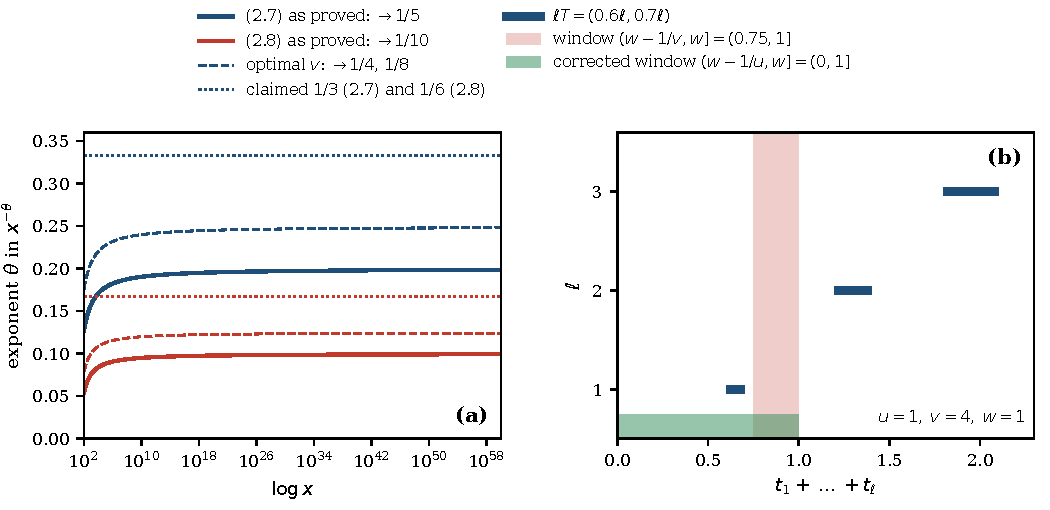
\includegraphics[width=\textwidth]{figures/fig_gkm_2015_audit.pdf}
\caption{(a) The exponent $\theta$ with $(v\log v)^{-v/2}=x^{-\theta}$ in (2.7) and (2.8) against
$\log x$, for $v=\log x/(2.5\log\log x)$ (solid) and for the largest admissible $v$ (dashed), with the
claimed values $\frac13$ and $\frac16$ (dotted). (b) The counterexample to Lemma~8.5: the sumsets $\ell T$
skip the window $(0.75,1]$, while the corrected window $(0,1]$ contains $T$.}\label{fig:main}
\end{figure}

\section{Lemma 8.5: the width of the window}\label{sec:85}

Lemma~8.5 (p.~25, stated without proof) reads as follows. Let $T$ be an open subset of
$(\frac1{ev},\frac1u]$. For any $w\ge1/v$ there is a positive integer $\ell\le evw$ such that
\[
\int\!\!\cdots\!\!\int_{\substack{w-1/v<t_1+\dots+t_\ell\le w\\ t_1,\dots,t_\ell\in T}}\frac{dt_1\cdots dt_\ell}{t_1\cdots t_\ell}
\ \ge\ \frac1{evw}\Bigl(\int_T\frac{dt}t\Bigr)^\ell .
\]
It is meant to be the continuous analogue of Lemma~7.1 and Corollary~7.2. In those results the steps lie
in $(y,z]$ and the window $(x-z,x]$ has width $z$, the maximal step. In Corollary~7.2 the steps are
$\log q\le\frac1u\log x$ and the window has logarithmic width $\frac1u$. In Lemma~8.5 the steps may be as
large as $\frac1u$, but the window has width only $\frac1v$. When $u<v$ the sums can jump over it. Probably $\frac1v$ in the window is a misprint for $\frac1u$, or
$\frac1u$ in the range of $T$ for $\frac1v$.

\emph{Counterexamples} ($u=1$, $v=4$, so $T\subset(0.092,1]$).
\begin{enumerate}
\item[(a)] $w=\frac12$ and $T=(0.55,0.9)$. Every sum of $\ell\ge1$ elements exceeds $0.55>w$, so the
left-hand side is $0$ for all $\ell$.
\item[(b)] $w=1$ and $T=(0.6,0.7)$. For $\ell=1$ the sums lie in $(0.6,0.7)$, below the window
$(0.75,1]$. For $\ell\ge2$ they exceed $1.2$. The left-hand side is again $0$ for all $\ell$, while the
right-hand side is positive (Figure~\ref{fig:main}(b)).
\end{enumerate}

\begin{lemma}[Lemma 8.5, corrected]\label{lem:85}
Let $0<a<b$, let $T\subset(a,b]$ be open with $\tau=\int_T dt/t>0$, and let $w\ge b$. Then there is a positive
integer $\ell\le w/a$ such that
\[
\int\!\!\cdots\!\!\int_{\substack{w-b<t_1+\dots+t_\ell\le w\\ t_1,\dots,t_\ell\in T}}\frac{dt_1\cdots dt_\ell}{t_1\cdots t_\ell}\ \ge\ \frac aw\,\tau^\ell .
\]
In particular, the conclusion of Lemma~8.5 holds (A) with the window $(w-\frac1u,w]$ for $w\ge\frac1u$
($a=\frac1{ev}$, $b=\frac1u$), and (B) as printed if $T\subset(\frac1{ev},\frac1v]$ and $w\ge\frac1v$
($a=\frac1{ev}$, $b=\frac1v$).
\end{lemma}

\begin{proof}
Let $\mu$ be the measure $dt/t$ on $T$, $K=\lfloor w/a\rfloor\ge1$, and $s_k=t_1+\dots+t_k$ for
$(t_1,\dots,t_K)\in T^K$. Then $s_1\le b\le w$, $s_K>Ka>w-a>w-b$, and $s_k-s_{k-1}\le b$. So the first
$k$ with $s_k>w-b$ satisfies $s_k\le w$: either $k=1$, or $s_k\le s_{k-1}+b\le w$. Integrating
$\sum_{k\le K}\mathbf 1[w-b<s_k\le w]\ge1$ against $\mu^K$ and dividing by $\tau^K$ gives $\sum_{k\le K}\beta_k\ge1$, where $\beta_k$
is the left-hand side for $\ell=k$ divided by $\tau^k$. Hence $\max_k\beta_k\ge1/K\ge a/w$.
\end{proof}

Proposition~8.4 concerns $T\subset(\frac1{ev},\frac1v]$, so version~(B) is exactly what its proof needs.
Proposition~8.4 is therefore unaffected. In $60$ random tests (unions of intervals, random $u<v$ and
$w\ge1/u$) a numerical convolution confirms version~(A). The smallest ratio of $\max_\ell\beta_\ell$ to
$1/(evw)$ observed was $3.5$.

\section{Two further remarks}\label{sec:further}

\emph{Hypothesis P $\Rightarrow$ Hypothesis A (p.~15).} Given $A\subset(\frac N{ev},\frac Nu]$, the proof
sets $\cP=\bigcup_{a\in A}\{p\in(e^a,e^{a+1})\}$ and $x=e^{[N]+1}$, and then applies Hypothesis~P, which
requires $\cP\subset(x^{1/ev},x^{1/u}]$. This can fail at both ends.
\begin{itemize}
\item \emph{Upper end.} If $a\in A$ with $a+1>([N]+1)/u$, primes up to $e^{a+1}>x^{1/u}$ occur. This needs
$u>1$, and at most one integer $a\le N/u$ qualifies.
\item \emph{Lower end.} If $a\in A$ with $a<([N]+1)/ev$, primes below $x^{1/ev}$ occur. At most one integer
in $(N/ev,([N]+1)/ev)$ qualifies.
\end{itemize}
For example, $N=1000$, $u=3$, $v=4$ gives $a=333$ and $a=92$. Removing these (at most two) elements before
defining $\cP$ changes $\sum_{a\in A}1/a$ by at most $2ev/N$. Since $u\le v$, this is
$O(v^2/N)\cdot\frac1u$, and it is absorbed by the factor $1+O(v^2/N)$ already present. The proof then goes
through unchanged.

\emph{Proposition~8.1 (p.~24).} With $w=(1+\lambda_1)/\sigma$, the proof replaces
$\sigma^{\ell+m}/(w^{O(w)}v(\ell+m)!)$ by $\sigma^{k+O(1/\sigma)}/(k\cdot k!)$, citing
$w\log w\ll\sigma^{-1}\log(1/\sigma)$. Since $\sigma\le1+o(1)$ and $\sigma$ may be close to $1$, this
inequality is false: as $\sigma\to1$ the right side tends to $0$, while $w\log w\to(1+\lambda_1)\log(1+\lambda_1)$.
For $\lambda_1=1$ and $\sigma=0.999$ the two sides are $1.39$ and $0.001$. The correct bound is
$w\log w\ll\sigma^{-1}(1+\log(1/\sigma))$. For $\sigma\ge\frac12$ this gives $w^{O(w)}=O(1)$, which is
absorbed into the implied constant. For $\sigma<\frac12$ we have $1\le\log(1/\sigma)/\log2$, and the
paper's bound follows. So Proposition~8.1 holds as stated. Table~\ref{tab:sum} summarises all points.

\begin{table}[ht]
\centering\footnotesize
\caption{Status of the points checked in \cite{GKMat} (arXiv page numbers).}\label{tab:sum}
\begin{tabular}{lll}
\toprule
Location & Issue & Status after repair\\
\midrule
Prop.~2.6, (2.7), p.~11 & $x^{-1/3}$ claimed; proof gives $x^{-1/5+o(1)}$ & Proposition~\ref{prop:26}\\
Prop.~2.6, (2.8), p.~11 & $x^{-1/6}$ claimed; proof gives $x^{-1/10+o(1)}$ & $x^{-1/8+\epsilon}$ with optimal $v$\\
Lemma~8.5, p.~25 & window $(w-\frac1v,w]$ too narrow; false as printed & Lemma~\ref{lem:85}; Prop.~8.4 unaffected\\
P $\Rightarrow$ A, p.~15 & $\cP$ may leave $(x^{1/ev},x^{1/u}]$ & remove $\le2$ elements of $A$\\
Prop.~8.1, p.~24 & $w\log w\ll\sigma^{-1}\log(1/\sigma)$ false as $\sigma\to1$ & conclusion holds as stated\\
\bottomrule
\end{tabular}
\end{table}

\FloatBarrier
\begin{thebibliography}{9}
\bibitem{GKMat} A.~Granville, D.~Koukoulopoulos and K.~Matom\"aki, \emph{When the sieve works}, Duke
Math.\ J.\ \textbf{164} (2015), no.~10, 1935--1969,
\href{https://doi.org/10.1215/00127094-3120891}{doi:10.1215/00127094-3120891}; arXiv:1205.0413.
\end{thebibliography}
\end{document}
